\begin{figure}
	\centering
	\begin{subfigure}{\textwidth}
		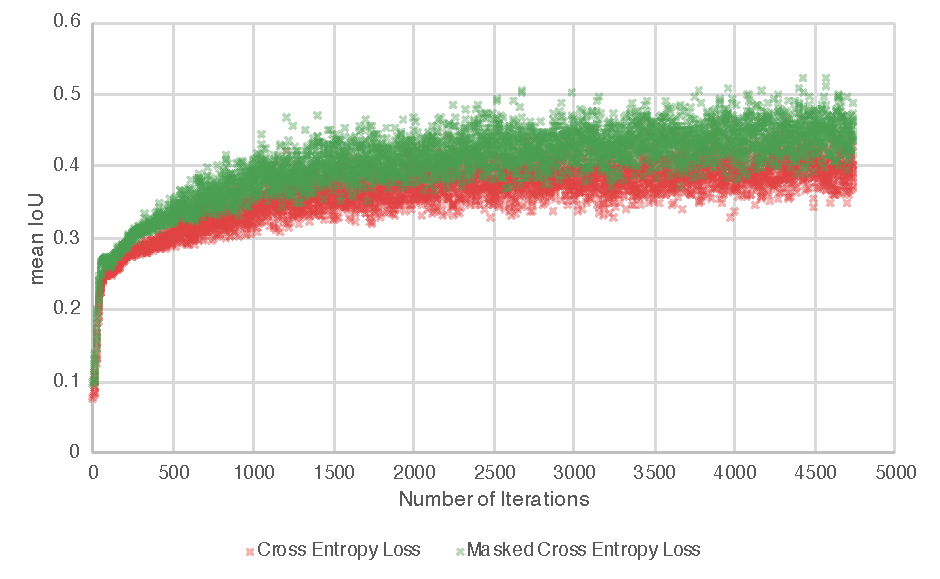
\includegraphics[width=\textwidth]{figures/experiments/loss-comparison-training.pdf}
		\caption[Loss Comparison Chart: Training]{Training mIoU Accuracy over 4740 Iterations comparing weighted cross entropy loss and masked cross entropy loss. The results show that although performing similarly to begin with, masked cross entropy loss was able to outperform weighted cross entropy loss.}
		\label{chart:experiments-losstraining}
	\end{subfigure}
	\newline
	\begin{subfigure}{\textwidth}
		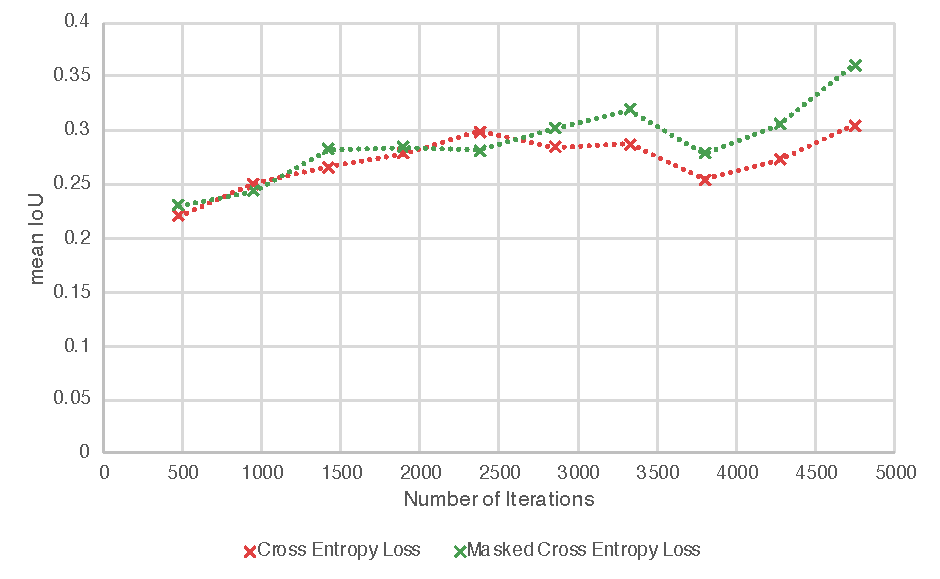
\includegraphics[width=\textwidth]{figures/experiments/loss-comparison-validation.pdf}
		\caption[Loss Comparison Chart: Validation]{Validation mean IoU Accuracy over 4740 Iterations, measured every 474 iterations, comparing cross entropy loss and masked cross entropy loss. Validation accuracy was evaluated against a validation set of 1680 images. The lines shown in the chart are to emphasize the data.}
		\label{chart:experiments-lossvalidation}
	\end{subfigure}
	\caption[Loss Comparison Chart]{Comparisons of masked cross entropy loss and weighted cross entropy loss. Both loss functions were evaluated using the same hyperparameters against a dataset consisting of 15160 training images and 1680 validation images.}
\end{figure}